%%%%(c) COPYRIGHT NOTICE%FOLDUP
%%%%(c)
%%%%(c)  This file is a portion of the source for the textbook
%%%%(c)
%%%%(c)    Numerical Methods Course Notes,
%%%%(c)    Copyright 2004-2010 by Steven E. Pav
%%%%(c)
%%%%(c)  See the file COPYING.txt for copying conditions
%%%%(c)
%%%%(c)%UNFOLD

%%throat clearing%FOLDUP
\typeout{-- matlab.tex}
\typeout{-- N� 2004-2010 Steven E. Pav}
%UNFOLD

%%local commands%FOLDUP
%UNFOLD

\chapter{A ``Crash'' Course in \octmat}
%%%%%%%%%%%%%%%%%%%%%%%%%%%%%%%%%%%%%%%%%%%%%%%
\section{Getting Started}%FOLDUP

Matlab is a software package that allows you to program the mathematics of an
algorithm without getting too bogged down in the details of data structures, 
pointers, and reinventing the wheel. It also includes graphing capabilities,
and there are numerous packages available for all kinds of functions, enabling
relatively high-level programming.  Unfortunately, it also costs quite a bit
of money, which is why I recommend the free Matlab clone, octave, available
under the GPL\footnote{Gnu Public License. See
\texttt{http://www.gnu.org/copyleft/gpl.html}.}, freely downloadable from 
\texttt{http://www.octave.org}.

In a lame attempt to retain market share, Mathworks continues to tinker with
Matlab to make it noncompatible with octave; this has the side effect of
obsoletizing old Matlab code.  I will try to focus on the intersection of the 
two systems, except where explicitly noted otherwise. What follows, then, is an
introduction to octave; Matlab users will have to make some changes.

You can find a number of \octmat tutorials for free on the web;  many of
them are certainly better than this one.  A brief web search reveals the
following excellent tutorials:
\begin{compactitem}
\item \texttt{http://www.math.mtu.edu/\~{}msgocken/intro/intro.html}
%available as postscript from
%\texttt{http://www.math.mtu.edu/\~{}msgocken/intro/intro.ps}.
\item \texttt{http://www.cyclismo.org/tutorial/matlab/vector.html}
\item \texttt{http://web.ew.usna.edu/\~{}mecheng/DESIGN/CAD/MATLAB/usna.html}
\end{compactitem}

Matlab has some demo programs covering a number of topics--
from the most basic functionality to the more arcane toolboxes.  In Matlab,
simply type \texttt{demo}.

What follows is a lame demo for octave.  Start up octave.  You 
should get something like:
\begin{verbatim}
GNU Octave, version 2.1.44 (i686-pc-linux-gnu).
Copyright (C) 1996, 1997, 1998, 1999, 2000, 2001, 2002, 2003 John W. Eaton.
This is free software; see the source code for copying conditions.
There is ABSOLUTELY NO WARRANTY; not even for MERCHANTIBILITY or
FITNESS FOR A PARTICULAR PURPOSE.  For details, type `warranty'.

Please contribute if you find this software useful.
For more information, visit http://www.octave.org/help-wanted.html

Report bugs to <bug-octave@bevo.che.wisc.edu>.

octave:1>
\end{verbatim}

You now have a command line.  The basic octavian data structure is a matrix; a
scalar is a $1\cross1$ matrix, a vector is an $n\cross1$ matrix.  
Some simple matrix constructions are as follows:
\begin{verbatim}
octave:2> a = [1 2 3]
a =

  1  2  3

octave:3> b = [5;4;3]
b =
  5
  4
  3

octave:4> c = a'
c =
  1
  2
  3

octave:5> d = 5*c - 2 * b
d =
  -5
   2
   9
\end{verbatim}

You should notice that octave ``echoes'' the lvalues it creates.  This is
either a feature or an annoyance.  It can be prevented by appending a semicolon
at the end of a command.  Thus the previous becomes

\begin{verbatim}
octave:5> d = 5*c - 2 * b;
octave:6> 
\end{verbatim}

For illustration purposes, I am leaving the semicolon off.  To access an entry
or entries of a matrix, use parentheses.   In the case where the variable is a
vector, you only need give a single index, as shown below;  when the variable is a
matrix, you need give both indices.  You can also give a range of indices, as
in what follows.

{\bf WARNING:} vectors and matrices in \octmat are indexed starting from $1,$
and \emph{not} from $0,$ as is more common in modern programming languages.
You are warned!  Moreover, the last index of a vector is denoted by the special 
symbol \texttt{end}.

\begin{verbatim}

octave:6> a(1) = 77
a =
  77   2   3

octave:7> a(end) = -400
a =
  77     2  -400

octave:8> a(2:3) = [22 333]
a =
   77   22  333

octave:9> M = diag(a)
M =
   77    0    0
    0   22    0
    0    0  333

octave:10> M(2,1) = 14
M =
   77    0    0
   14   22    0
    0    0  333

octave:11> M(1:2,1:2) = [1 2;3 4]
M =
    1    2    0
    3    4    0
    0    0  333
\end{verbatim}
The command \texttt{diag(v)} returns a matrix with \texttt{v} as the diagonal,
if \texttt{v} is a vector.  \texttt{diag(M)} returns the diagonal of matrix
\texttt{M} as a vector.

The form \texttt{c:d} gives returns a row vector of the integers between
\texttt{a} and \texttt{d}, as we will examine later.  First we look at 
matrix manipulation:
\begin{verbatim}
octave:12> j = M * b
j =
   13
   31
  999

octave:13> N = rand(3,3)
N =
  0.166880  0.027866  0.087402
  0.706307  0.624716  0.067067
  0.911833  0.769423  0.938714

octave:14> L = M + N
L =
    1.166880    2.027866    0.087402
    3.706307    4.624716    0.067067
    0.911833    0.769423  333.938714

octave:15> P = L * M
P =
   7.2505e+00   1.0445e+01   2.9105e+01
   1.7580e+01   2.5911e+01   2.2333e+01
   3.2201e+00   4.9014e+00   1.1120e+05

octave:16> P = L .* M
P =
   1.1669e+00   4.0557e+00   0.0000e+00
   1.1119e+01   1.8499e+01   0.0000e+00
   0.0000e+00   0.0000e+00   1.1120e+05

octave:17> x = M \ b
x =
  -6.0000000
   5.5000000
   0.0090090

octave:18> err = M * x - b
err =
  0
  0
  0
\end{verbatim}

Note the difference between \texttt{L * M} and \texttt{L .* M};  the former is
matrix multiplication, the latter is \emph{element by element} multiplication,
\ie $$\Parens{\mathtt{L\, .\!* M}}_{i,j} = \mathtt{L}_{i,j}\,\mathtt{M}_{i,j}.$$
The command \texttt{rand(m,n)} gives an $m\cross n$ matrix with each element
``uniformly distributed'' on \ccinv{0}{1}. 
For a zero mean normal distribution with unit variance, use \texttt{randn(m,n)}.

In line 17 we asked octave to solve the linear system
$$\mathtt{M} \mathtt{x} = \mathtt{b},$$
by setting
$$\mathtt{x} = \mathtt{M} \backslash \mathtt{b} = \mathtt{M}^{-1} \mathtt{b}.$$

Note that you can construct matrices directly as you did vectors:
\begin{verbatim}
octave:19> B = [1 3 4 5;2 -2 2 -2]
B =
   1   3   4   5
   2  -2   2  -2
\end{verbatim}
You can also create row vectors as a sequence, either using the form
\texttt{c:d} or the form \texttt{c:e:d}, which give, respectively, 
$\mathtt{c},\mathtt{c}+1,\ldots,\mathtt{d},$ and 
$\mathtt{c},\mathtt{c}+\mathtt{e},\ldots,\mathtt{d},$
(or something like it if $\mathtt{e}$ does not divide $\mathtt{d}-\mathtt{c}$)
%$\mathtt{c},\mathtt{c}+\mathtt{e},\ldots,\mathtt{c} +
%\floor{({\mathtt{d} - \mathtt{c}})/{\mathtt{e}}} \mathtt{e}$
as follows:

\begin{verbatim}
octave:20> z = 1:5
z =
  1  2  3  4  5

octave:21> z = 5:(-1):1
z =
  5  4  3  2  1

octave:22> z = 5:(-2):1
z =
  5  3  1

octave:23> z = 2:3:11
z =
   2   5   8  11

octave:24> z = 2:3:10
z =
   2   5   8
\end{verbatim}
Matrices and vectors can be constructed ``blockwise.'' Blocks in the same row
are separated by a comma, those in the same column by a semicolon.  Thus
\begin{verbatim}
octave:2> y=[2 7 9]
y =
  2  7  9

octave:3> m = [z;y]
m =
  2  5  8
  2  7  9

octave:4> k = [(3:4)', m]
k =
  3  2  5  8
  4  2  7  9

\end{verbatim}


%UNFOLD
%%%%%%%%%%%%%%%%%%%%%%%%%%%%%%%%%%%%%%%%%%%%%%%
\section{Useful Commands}%FOLDUP

Here's a none too complete listing of useful commands in octave:

\begin{compactitem}
\item \texttt{help} is the most useful command.
\item \texttt{floor(X)} returns the largest integer not greater than \texttt{X}.
If \texttt{X} is a vector or matrix, it computes the floor element-wise.  This
behavior is common in octave: many functions which we normally think of as
applicable to scalars can be applied to matrices, with the result computed
element-wise.
\item \texttt{ceil(X)} returns the smallest integer not less than \texttt{X},
computed element-wise.
\item \texttt{sin(X)},
\texttt{cos(X)},
\texttt{tan(X)},
\texttt{atan(X)},
\texttt{sqrt(X)},
 returns the sine, cosine, tangent, arctangent, square root of \texttt{X}, 
 computed elementwise.
\item \texttt{exp(X)} returns $\exp{\mathtt{X}},$ elementwise.
\item \texttt{abs(X)} returns $\abs{\mathtt{X}},$ elementwise.
\item \texttt{norm(X)} returns the norm of \texttt{X};  if \texttt{X} is a
vector, this is the \Ltwo[]{} norm:
$$\dltwo{\mathtt{X}} = \Parens{\sum_i \mathtt{X}_i^2 }^{1/2},$$
if \texttt{X} is a matrix, it is the matrix norm subordinate to the \Ltwo[]{}
norm.

You can compute other norms with \texttt{norm(X,p)} where \texttt{p} is a
number, to get the \Lp[]{} norm, or with \texttt{p} one of
\texttt{Inf}, \texttt{-Inf}, etc.
\item \texttt{zeros(m,n)} returns an $m\cross n$ matrix of all zeros.
\item \texttt{eye(m)} returns the $m\cross m$ identity matrix.
\item \texttt{[m,n] = size(A)} returns the number of rows, columns of
\texttt{A}. Similarly the functions \texttt{rows(A)} and \texttt{columns(A)}
return the number of rows and columns, respectively.
\item \texttt{length(v)} returns the length of vector \texttt{v}, or the larger
dimension if \texttt{v} is a matrix.
\item \texttt{find(M)} returns the indices of the nonzero elements of
\texttt{N}.  This may not seem helpful at first, but it can be very useful for
selecting subsets of data because the indices can be used for selection.
Thus, for example, in this code
\begin{verbatim}
octave:1> v = round(20*randn(400,3));
octave:2> selectv = v(find(v(:,2) == 7),:)
\end{verbatim}
we have selected the rows of \texttt{v} where the element in the second column
equals $7$.  Now you see why leading computer scientists refer to \octmat as
``semantically suspect.''  It is a very useful language nonetheless, and you
should try to learn its quirks rather than resist them.
\item \texttt{diag(v)} returns the diagonal matrix with vector \texttt{v} as
diagonal.  
\texttt{diag(M)} returns as a vector, the diagonal of matrix \texttt{v}.
Thus \texttt{diag(diag(v))} is \texttt{v} for vector \texttt{v}, but 
\texttt{diag(diag(M))} is the diagonal part of matrix \texttt{M}.
\item \texttt{toeplitz(v)} returns the Toeplitz matrix associated with vector
\texttt{v}.  That is
\[
\mathtt{toeplitz(v)} = 
\left[\begin{array}{ccccc}
\mathtt{v(1)} & \mathtt{v(2)} & \mathtt{v(3)} & \cdots & \mathtt{v(n)}\\
\mathtt{v(2)} & \mathtt{v(1)} & \mathtt{v(2)} & \cdots & \mathtt{v(n-1)}\\
\mathtt{v(3)} & \mathtt{v(2)} & \mathtt{v(1)} & \cdots & \mathtt{v(n-2)}\\
\vdots & \vdots & \vdots & \ddots & \vdots\\
\mathtt{v(n)} & \mathtt{v(n-1)} & \mathtt{v(n-2)} & \cdots & \mathtt{v(1)}
\end{array}\right]
\]
In the more general form, \texttt{toeplitz(c,r)} can be used to return a
assymmetric Toeplitz matrix.

A matrix which is banded on the cross diagonals is evidently called a
``Hankel'' matrix:
\[
\mathtt{hankel(u,v)} = 
\left[\begin{array}{ccccc}
\mathtt{u(1)} & \mathtt{u(2)} & \mathtt{u(3)} & \cdots & \mathtt{u(n)}\\
\mathtt{u(2)} & \mathtt{u(3)} & \mathtt{u(4)} & \cdots & \mathtt{v(2)}\\
\mathtt{u(3)} & \mathtt{u(4)} & \mathtt{u(5)} & \cdots & \mathtt{v(3)}\\
\vdots & \vdots & \vdots &  & \vdots\\
\mathtt{u(n)} & \mathtt{v(2)} & \mathtt{v(3)} & \cdots & \mathtt{v(n)}
\end{array}\right]
\]

\item \texttt{eig(M)} returns the eigenvalues of \texttt{M}.
\texttt{[V, LAMBDA] = eig(M)} returns the eigenvectors, and eigenvalues of
\texttt{M}.
\item \texttt{kron(M,N)} returns the Kronecker product of the two matrices.
This is a blcok construction which returns a matrix where each block is an
element of \texttt{M} as a scalar multiplied by the whole matrix \texttt{N}.
\item \texttt{flipud(N)} flips the vector or matrix \texttt{N} so that its
first row is last and \vicev.  Similarly \texttt{fliplr(N)} flips left/right.
\end{compactitem}



%UNFOLD
%%%%%%%%%%%%%%%%%%%%%%%%%%%%%%%%%%%%%%%%%%%%%%%
\section{Programming and Control}%FOLDUP

If you are going to do any serious programming in octave, you should keep
your commands in a file.  octave loads commands from `.m' files.\footnote{The `m'
stands for `octave.'}  If you have the following in a file called
\texttt{myfunc.m}:
\begin{verbatim}
function [y1,y2] = myfunc(x1,x2)
% comments start with a `%'
% this function is useless, except as an example of functions.
% input:
%  x1			a number
%  x2			another number
% output:
%  y1			some output
%  y2			some output

y1 = cos(x1) .* sin(x2);
y2 = norm(y1);
\end{verbatim}
then you can call this function from octave, as follows:
\begin{verbatim}
octave:1> myfunc(2,3)
ans = -0.058727
octave:2> [a,b] = myfunc(2,3)
a = -0.058727
b = 0.058727
octave:3> [a,b] = myfunc([1 2 3 4],[1 2 3 4])
a =

   0.45465  -0.37840  -0.13971   0.49468

b = 0.78366
\end{verbatim}
Note this silly function will throw an error if \texttt{x1} and \texttt{x2} are
not of the same size.

It is recommended that you write your functions so that they can take scalar
and vector input where appropriate.  For example, the octave builtin sine
function can take a scalar and output a scalar, or take a vector and output a
vector which is, elementwise, the sine of the input.  It is not too difficult
to write functions this way, it often only requires judicious use of
\texttt{.*} multiplies instead of \texttt{*} multiplies.  For example, if the
file \texttt{myfunc.m} were changed to read
\begin{verbatim}
y1 = cos(x1) * sin(x2);
\end{verbatim}
it could easily crash if \texttt{x1} and \texttt{x2} were vectors of the same
size because matrix multiplication is not defined for an $n\cross1$ matrix
times another $n\cross1$ matrix.

An .m file does not have to contain a function, it can merely contain some
octave commands.  For example, putting the following into 
\texttt{runner.m}:
\begin{verbatim}
x1 = rand(4,3);
x2 = rand(size(x1));
[a,b] = myfunc(x1,x2)
\end{verbatim}
octave allows you to call this script without arguments:
\begin{verbatim}
octave:4> runner
a =

  0.245936  0.478054  0.535323
  0.246414  0.186454  0.206279
  0.542728  0.419457  0.083917
  0.257607  0.378558  0.768188

b = 1.3135
\end{verbatim}

octave has to know where your .m file is.  It will look in the directory from
which it was called.  You can set this to something else with \texttt{cd} or
\texttt{chdir}.

You can also use the octave builtin function \texttt{feval} to evaluate a
function by name.  For example, the following is a different way of calling
\texttt{myfunc.m}:
\begin{verbatim}
octave:5> [a,b] = feval("myfunc",2,3)
a = -0.058727
b = 0.058727
\end{verbatim}
In this form \texttt{feval} seems like a way of using more keystrokes to get
the same result. However, you can pass a variable function name as well:
\begin{verbatim}
octave:6> fname = "myfunc"
fname = myfunc
octave:7> [a,b] = feval(fname,2,3)
a = -0.058727
b = 0.058727
\end{verbatim}
This allows you to effectively pass functions to other functions.

\subsection{Logical Forks and Control}

octave has the regular assortment of `if-then-else' and `for' and `while'
loops.  These take the following form:
%\begin{table}[h]%FOLDUP
%\begin{center}
%\begin{tabular}{|l|l|l|}
%\hline
%\begin{verbatim}
%if expr1
%  statements
%elseif expr2
%  statements
%elsif expr3
%  statements
%...
%else
%  statements
%end
%\end{verbatim}
%&
%\begin{verbatim}
%for var=vector
%  statements
%end
%\end{verbatim}
%&
%\begin{verbatim}
%while expr
%  statements
%end
%\end{verbatim}
%\hline
%\end{tabular}
%\end{center}
%\caption{caption}\label{tab:atable}
%\end{table}%UNFOLD
%\begin{minipage}[c][0.8\columnwidth][c]{0.10\columnwidth}
\begin{verbatim}
if expr1
  statements
elseif expr2
  statements
elsif expr3
  statements
...
else
  statements
end
for var=vector
  statements
end
while expr
  statements
end
\end{verbatim}
%\end{minipage}

Note that the word \texttt{end} is one of the most overloaded in \octmat.  It stands
for the last index of a vector of matrix, as well as the exit point for for
loops, if statements, switches, etc. To simplify debugging, it is also
permissible to use \texttt{endif} to end an \texttt{if} statement,
\texttt{endfor} to end a \texttt{for} loop, \etc.

The test expressions may use the logical conditionals:
\texttt{>}, \texttt{<}, \texttt{>=}, \texttt{<=}, \texttt{==}, \texttt{\~{}=}.
Do \emph{not} use the assignment operator \texttt{=} as a conditional, as this
can lead to disastrous results, as in C.

Here are some examples:
\begin{verbatim}
%compute the sign of x
if x > 0
  s = 1;
elseif x == 0
  s = 0;
else
  s = -1;
end

%a `regular' for loop
for i=1:10
  sm = sm + i;
end

%an `irregular' for loop
for i=[1 2 3 5 8 13 21 34]
  fsm = fsm + i;
end

while (sin(x) > 0)
  x = x * pi;
end
\end{verbatim}
%UNFOLD
%%%%%%%%%%%%%%%%%%%%%%%%%%%%%%%%%%%%%%%%%%%%%%%
\section{Plotting}%FOLDUP
Plotting is one area in which there are some noticeable differences between
octave and Matlab.  The commands and examples given herein are for octave, but
the commands for Matlab are not too different.
octave ships its plotting commands to Gnuplot.

The main plot command is \texttt{plot}.  You may also use \texttt{semilogx},
\texttt{semilogy},\texttt{loglog} for 2D plots with log axes, and
\texttt{contour} and \texttt{mesh} for 3D plots.  Use the \texttt{help} command
to get the specific syntax for each command.  We present some examples:

\begin{verbatim}
n = 100;
X = pi .* ((1:n) ./ n);
Y = sin(X);
%just plot Y
plot(Y);
%plot Y, but with the `right' X axis labels
plot(X,Y);

W = sqrt(Y);
plot(W);
%plot W, but with the `right' X axis labels
plot(Y,W);
\end{verbatim}

The output from these commands is seen in \figref{octaveplots}.  In particular,
you should note the difference between plotting a vector, as in
\figref{subfigc} versus plotting the same vector but with the appropriate
abscissa values, as in \figref{subfigd}.

\begin{figure}[htp]
\centering
%\subfigure[$Y = sin(X)$]{
\subfloat[$Y = sin(X)$]{
		\label{fig:subfiga}
		\includegraphics[width=.31\columnwidth,angle=270]{justy.ps}}
\hspace{.3in}
%\subfigure[$Y$ versus $X$]{
\subfloat[$Y$ versus $X$]{
		\label{fig:subfigb}
		\includegraphics[width=.31\columnwidth,angle=270]{xandy.ps}}
\vspace{.3in}
%\subfigure[$W = \sqrt{Y}$]{
\subfloat[$W = \sqrt{Y}$]{
		\label{fig:subfigc}
		\includegraphics[width=.31\columnwidth,angle=270]{justw.ps}}
\hspace{.3in}
%\subfigure[$W$ versus $Y$]{
\subfloat[$W$ versus $Y$]{
		\label{fig:subfigd}
		\includegraphics[width=.31\columnwidth,angle=270]{yandw.ps}}
\caption{Four plots from octave.} \label{fig:octaveplots}
\end{figure}



Some magic commands are required to plot to a file.  For octave, I recommend
the following magic formula, which replots the figure to a file:
\begin{verbatim}
%call the plot commands before this line
gset term postscript color;			
gset output "filename.ps";
replot;
gset term x11;
gset output "/dev/null";
\end{verbatim}

In Matlab, the commands are something like this:
\begin{verbatim}
%call the plot commands before this line
print(gcf,'-deps','filename.eps');
\end{verbatim}

%UNFOLD
%%%%%%%%%%%%%%%%%%%%%%%%%%%%%%%%%%%%%%%%%%%%%%%
%\section{Exercises}%FOLDUP
\begin{bkexs}
%%%%%%%%%%%%%%%%%%%%%%%%%%%%%%%%
\item What do the following pieces of \octmat code accomplish?
\begin{compactenum}
\item \begin{verbatim}x = (0:40) ./ 40;\end{verbatim}
\item \begin{verbatim}a = 2;
b = 5;
x = a + (b-a) .* (0:40) ./ 40;\end{verbatim}
\item \begin{verbatim}x = a + (b-a) .* (0:40) ./ 40;
y = sin(x);
plot(x,y);\end{verbatim}
\end{compactenum}

%%%%%%%%%%%%%%%%%%%%%%%%%%%%%%%%
\item Implement the \naive quadratic formula to find the roots of $x^2 + bx +
c = 0,$ for real $b,c.$  Your code should return
$$\frac{-b \pm \sqrt{b^2 - 4 c}}{2}.$$
Your m-file should have header line like:
\begin{verbatim}
function [x1,x2] = naivequad(b,c)
\end{verbatim}
Test your code for $\tuple{b,c} = \tuple{\tenex{1}{15},1}.$  Do you get a
spurious root?
%%%%%%%%%%%%%%%%%%%%%%%%%%%%%%%%
\item Implement a robust quadratic formula (\cf \bkexpref{quadratic}) to find
the roots of $x^2 + bx + c = 0.$
Your m-file should have header line like:
\begin{verbatim}
function [x1,x2] = robustquad(b,c)
\end{verbatim}
Test your code for $\tuple{b,c} = \tuple{\tenex{1}{15},1}.$  Do you get a
spurious root?
%%%%%%%%%%%%%%%%%%%%%%%%%%%%%%%%
\item Write \octmat code to find a fixed point for the cosine, \ie some $x$
such that $x = \cos(x).$  Do this as follows: pick some initial value $x_0,$
then let $x_{i+1} = \cos(x_{i})$ for $i=0,1,\ldots,n.$  Pick $n$ to be
reasonably large, or choose some convergence criterion (\ie terminate if $\abs{x_{i+1} -
x_i} < \tenex{1}{-10}$).  Does your code always converge?
%%%%%%%%%%%%%%%%%%%%%%%%%%%%%%%%
\item The centered \emph{sigmoidal function} is used in neural nets, and is 
defined as
\[\sigma(x) = \frac{1-\exp{-x}}{1 + \exp{-x}}\]
Implement this function in \octmat.  
Your m-file should have header line like:
\begin{verbatim}
function sigx = sigmoidal(x)
\end{verbatim}
Test your code on $x=0,1,100,\tenex{1}{5},-100,\tenex{-1}{5}$.
Does something bad happen for $x=\tenex{-1}{5}$?  Is this a problem of 
loss of significance?  Reimplement your code to make it robust against this
problem.  
\begin{bkhint}use the fact that $\sigma(x)$ is an odd function.
\end{bkhint}

%%%%%%%%%%%%%%%%%%%%%%%%%%%%%%%%
\item Write code to implement the factorial function for integers:
\begin{verbatim}
function [nfact] = factorial(n)
\end{verbatim}
where $n$ factorial is equal to $1 \cdot 2 \cdot 3 \cdots (n-1) \cdot n.$
Either use a `for' loop, or write the function to recursively call itself.
%\begin{verbatim}
%function [nfact] = factorialRec(n)
%if (n == 0) 
%  nfact = 1;
%else
%  nfact = n * factorialRec(n-1);
%end
%\end{verbatim}
\end{bkexs}
%UNFOLD
%for vim modeline: (do not edit)
% vim:ts=2:sw=2:tw=79:fdm=marker:fmr=FOLDUP,UNFOLD:cms=%%s:tags=tags;:syntax=tex:filetype=tex:ai:si:cin:nu:fo=croqt:cino=p0t0c5(0:
